\section{Introducción}

\section{Antecedentes}

¿Cómo se viene/venía realizando la gestión del POETY?¿Qué cuellos de botella presentaba? ¿Qué áreas de oportunidad se detectan de la evaluación del proceso?
\section{Descripción de Sistema (Alcances del Sistema)}

\subsection{Objetivos General del Sistema}

Los Objetivos del Negocio del proyecto del Sistema de gestión del POETY son:
\begin{itemize}
\item Proporcionar un mecanismo de conocimiento y soporte geográfico de decisiones para la gestión del POETY(QUÉ).
\item Desarrollando un Sistema que permita la gestión del POETY mediante la organización dinámica de información relevante, la simplificación de informes técnicos, al definirse como base para configuración de la bitácora ambiental, así como geovisualizaciones que faciliten los procesos multi-escalares, multitemporales y multi-sectoriales de la transformación territorial y la vulnerabilidad de los ecosistemas al cambio climático. (CÓMO)
\item Para que las autoridades así como otros actores de la vida pública cuenten con un mecanismo que funcione como un sistema de información geográfica para la puesta en marcha de la actualización del POETY, para el manejo, análisis y visualización de información que facilite la gobernanza colaborativa en el proceso de ordenamiento ecológico en la entidad y su articulación con otros instrumentos de planeación pertinentes.(POR QUÉ)
\end{itemize}

\pagebreak
\subsection{Requerimientos del Sistema}


\begin{longtable}{@{\extracolsep{2pt}}l p{7cm} p{5cm}}  
\caption{Requerimientos del Sistema}\label{item:req_sistema}\\
\\[-1.8ex]\hline 
\endhead
\hline \\[-1.8ex] 
 \multicolumn{1}{c} {\textit{\textbf{Num}}}& {\textit{\textbf{Requerimiento}}} & {\textit{\textbf{Descripción}}}\\ 
\hline \\[-1ex] 
\\
1 & Acceso interactivo a bancos de datos de la caracterización ambiental y socio-económica & \\
\\
\hline 
\\
2 & Monitoreo y evaluación pública a través de índices e indicadores del desempeño del ordenamiento ecológico & \\
\\
\hline 
\\
3 & Consulta interactiva de mecanismos de resolución de conflictos del programa de ordenamiento ecológico con base en los criterios, estrategias y lineamientos de regulación ecológico en cada UGA & \\
\\
\hline 
\\
4 & Simplificar la consulta de informes técnicos & \\
\\
\hline 
\\
5 & Permitir la realización de procedimientos de geovisualización que incluyan como mínimo manejo de bancos de datos, manejo de modelos de análisis, generador de reportes gráficos y tabulares e interfaces de operación & \\
\\
\hline 
\hline \\[-1.8ex] 
  \\ 
\end{longtable} 

\subsection{Beneficios}

\subsection{Limitaciones del sistema}


\section{Especificación de Requerimientos funcionales}

\subsection{Priorización de Requerimientos}

\newgeometry{hmargin=.4in,vmargin=0.1in} 

\begin{landscape}
\begin{figure}[h]

\centering
\caption{Priorización de requerimientos}\label{fig:priorReq}
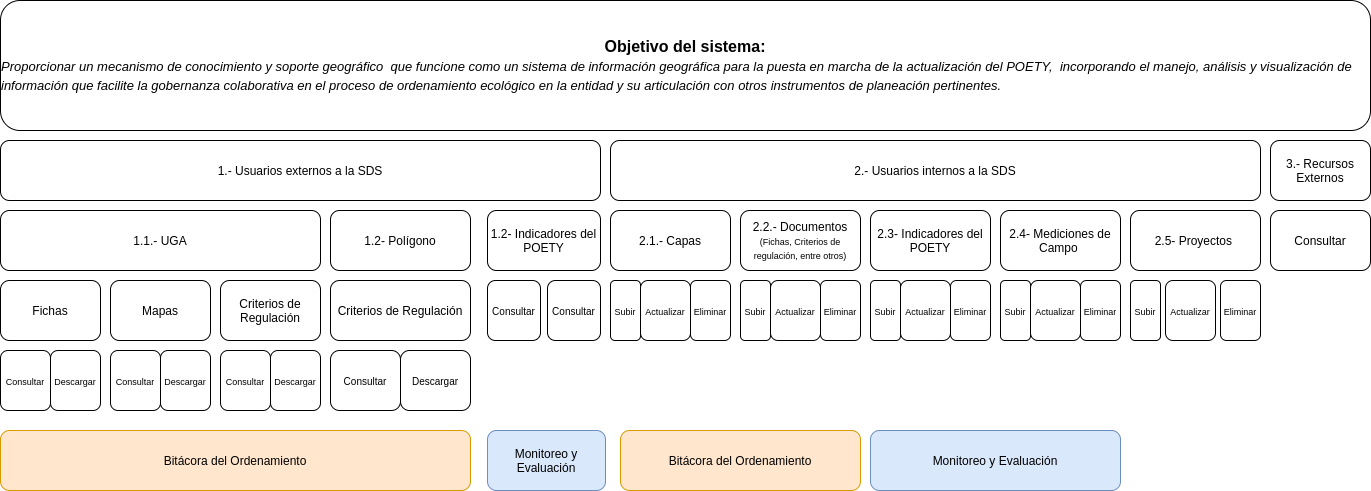
\includegraphics[width=1.5\textwidth, height=.7\textwidth]{images/PrioritizationRequirements.png}
\end{figure}
\end{landscape}
\restoregeometry

\subsection{Diagrama de Casos de Uso}

\subsection{Descripción de Módulos y Casos de Uso}


\begin{longtable}{@{\extracolsep{6pt}}l p{7.5cm}}  
\caption{Módulos y Casos de Uso}\label{item:mod_cu}\\
\\[-1.8ex]\hline 
\endhead
\hline \\[-1.8ex] 
 \multicolumn{1}{c} {\textit{\textbf{Módulo}}} & {\textit{\textbf{Casos de Uso}}} \\ 
\hline \\[-1ex] 

  & Consultar fichas de UGAs\\
\cline{2-2}
	 & Consultar fichas de UGAs\\
\cline{2-2}
	 & Descargar ficha de UGA\\
\cline{2-2}
	 & Consultar capas de insumo para el ordenamiento\\	 
\cline{2-2}
	 & Consultar mapas de aptitud\\
\cline{2-2}
	 & Consultar mapas de UGAs\\
\cline{2-2}
	 & Consultar documentos relacionados con la formulación del POETY\\	 
\cline{2-2}
	 & Consultar criterios de regulación por polígono\\	 
\cline{2-2}
Bitácora del ordenamiento	 & Descargar criterios de regulación por polígono\\	 
\cline{2-2}
	 & Descargar criterios de regulación por UGA\\	 
\cline{2-2}
	 & Subir documentos (fichas, u otros)\\	 
\cline{2-2}
	 & Subir capas \\	 
\cline{2-2}
	 & Actualizar documentos (fichas, u otros)\\	 
\cline{2-2}
	 & Actualizar capas \\	 
\cline{2-2}
	 & Borrar documentos (fichas, u otros)\\
\cline{2-2}
	 & Borrar capas \\	
\hline
	 & Subir mediciones de campo \\	
\cline{2-2}
	 & Actualizar mediciones de campo \\		 	  
\cline{2-2}
Monitoreo y evaluación	 & Borrar mediciones de campo\\	
\cline{2-2}
	 & Consultar indicadores del POETY \\	
\hline
	 & 
Obtener un informe sobre los criterios de regulación y los impactos acumulados\\	
\cline{2-2}
 &
LLenar un formulario cuando se dictamina un proyecto \\	
\cline{2-2}
Automatización de reportes	 & Modificar los datos de un proyecto \\	
\cline{2-2}
	 & Borrar proyectos en la base de datos de proyectos\\	
\cline{2-2}
	 & Obtener información externa y cruzarla con un polígono de interés \\	
\hline
	 &Dar de alta usuario interno de SDS \\	
\cline{2-2}
Módulo de administración	 & Dar de baja usuario interno de SDS  \\	
\cline{2-2}
	 & Modificar datos de usuarios internos de SDS\\	
 	 	 	 	 	 	 	 	 	 	 	 	 	 	 	 	 	 	 	 	 
\hline 
\hline \\[-1.8ex] 
  \\ 
\end{longtable} 

\pagebreak
\subsection{Casos de Uso}

%%%%%%%%%%%%%%%%%%%%%%%%%%%%%%%%%%%%%%%%%%%%%%%%%%%%%%%%%%
%%%%%% CU: Subir mediciones de campo
%%%%%%%%%%%%%%%%%%%%%%%%%%%%%%%%%%%%%%%%%%%%%%%%%%%%%%%%%%

\begin{longtable}{@{\extracolsep{8pt}}l p{8.5cm}}  
\caption{Caso de uso: Subir mediciones de campo}\label{item:subir_mediciones_campo}\\
\\[-1.8ex]\hline 
\endhead
\hline \\[-1.8ex] 
 \multicolumn{1}{c} {\textit{\textbf{CASO DE USO}}}& {\textit{\textbf{Subir mediciones de campo}}} \\ 
\hline \\[-1ex] 
ID. DEL CU&   \\
\hline\\[-1ex] 
ACTORES PARTICIPANTES & Usuario interno de SDS\\
\hline \\[-1ex] 
BREVE DESCRIPCIÓN & El funcionario incorpora las mediciones de campo al sistema.\\
\hline \\[-1ex] 

PRE-CONDICIONES & \textbf{Del proceso}: \par\vspace{.1cm} NA.
 \par\vspace{.2cm} \textbf{Del sistema} \par\vspace{.1cm} El actor debe estar autenticado como usuario interno de la SDS.\\
\hline \\[-1ex] 

FLUJO PRINCIPAL & 
1.- El usuario ingresa sus credenciales de usuario: nombre de usuario y contraseña.(A1).
\par\vspace{.1cm} 2.- El usuario se dirige al apartado de “registrar mediciones”.
\par\vspace{.1cm} 3.- El Sistema muestra una forma de registro de la medición y el usuario la llena.
\par\vspace{.1cm} 4.- El usuario registra los datos de la  medición y elige la opción “Registrar Medición”.
\par\vspace{.1cm} 5.- El Sistema muestra una advertencia de registro de la medición
\par\vspace{.1cm} 6.- El usuario acepta la advertencia.(A2)
\par\vspace{.1cm} 7.- El sistema registra los datos de la medición.(E1)

\\
\hline \\[-1ex] 

FLUJOS ALTERNOS & (A1)En caso de no contar con credenciales, ver caso de uso Dar de alta usuario.
\par\vspace{.1cm} (A2) En caso contrario, el usuario sale del proceso.
\\
\hline \\[-1ex] 

FLUJOS DE EXCEPCIÓN & (E1). El sistema no puede acceder a la bd\\
\hline \\[-1ex] 
POST-CONDICIONES & La medición de campo queda efectivamente registrada en la bd.\\

 
\hline 
\hline \\[-1.8ex] 
  \\ 
\end{longtable} 

%%%%%%%%%%%%%%%%%%%%%%%%%%%%%%%%%%%%%%%%%%%%%%%%%%%%%%%%%%
%%%%%% CU: Actualizar mediciones de campo
%%%%%%%%%%%%%%%%%%%%%%%%%%%%%%%%%%%%%%%%%%%%%%%%%%%%%%%%%%
\pagebreak
\begin{longtable}{@{\extracolsep{8pt}}l p{8.5cm}}  
\caption{Caso de uso: Actualizar mediciones de campo}\label{item:actualizar_mediciones_campo}\\
\\[-1.8ex]\hline 
\endhead
\hline \\[-1.8ex] 
 \multicolumn{1}{c} {\textit{\textbf{CASO DE USO}}}& {\textit{\textbf{Actualizar mediciones de campo}}} \\ 
\hline \\[-1ex] 
ID. DEL CU&   \\
\hline\\[-1ex] 
ACTORES PARTICIPANTES & Usuario interno de SDS\\
\hline \\[-1ex] 
BREVE DESCRIPCIÓN & El funcionario actualiza las mediciones de campo al sistema.\\
\hline \\[-1ex] 

PRE-CONDICIONES & \textbf{Del proceso}: \par\vspace{.1cm} Debe existir la medición a modificar.
 \par\vspace{.2cm} \textbf{Del sistema} \par\vspace{.1cm} El actor debe estar autenticado como usuario interno de la SDS.\\
\hline \\[-1ex] 

FLUJO PRINCIPAL & 
1.- El usuario ingresa sus credenciales de usuario: nombre de usuario y contraseña.(A1).
\par\vspace{.1cm} 2.- El usuario se dirige al apartado de “actualizar mediciones”.
\par\vspace{.1cm} 3.- El usuario ingresa el id de la medición.(E1)
\par\vspace{.1cm} 4.- El Sistema muestra una forma de actualización de la medición y el usuario la llena.
\par\vspace{.1cm} 5.- El usuario registra los datos de la  medición y elige la opción “Registrar Medición”.
\par\vspace{.1cm} 6.- El Sistema muestra una advertencia de actualización de la medición.
\par\vspace{.1cm} 7.- El usuario acepta la advertencia.(A2)
\par\vspace{.1cm} 8.- El sistema registra los datos actualizados de la medición.(E1)

\\
\hline \\[-1ex] 

FLUJOS ALTERNOS & (A1)En caso de no contar con credenciales, ver caso de uso Dar de alta usuario.
\par\vspace{.1cm} (A2) En caso contrario, el usuario sale del proceso.
\\
\hline \\[-1ex] 

FLUJOS DE EXCEPCIÓN & (E1). El sistema no puede acceder a la bd\\
\hline \\[-1ex] 
POST-CONDICIONES & La actualización de la medición de campo queda efectivamente registrada en la bd.\\

 
\hline 
\hline \\[-1.8ex] 
  \\ 
\end{longtable} 

%%%%%%%%%%%%%%%%%%%%%%%%%%%%%%%%%%%%%%%%%%%%%%%%%%%%%%%%%%
%%%%%% CU: Borrar mediciones de campo
%%%%%%%%%%%%%%%%%%%%%%%%%%%%%%%%%%%%%%%%%%%%%%%%%%%%%%%%%%
\pagebreak
\begin{longtable}{@{\extracolsep{8pt}}l p{8.5cm}}  
\caption{Caso de uso: Borrar mediciones de campo}\label{item:borrar_mediciones_campo}\\
\\[-1.8ex]\hline 
\endhead
\hline \\[-1.8ex] 
 \multicolumn{1}{c} {\textit{\textbf{CASO DE USO}}}& {\textit{\textbf{Borrar mediciones de campo}}} \\ 
\hline \\[-1ex] 
ID. DEL CU&   \\
\hline\\[-1ex] 
ACTORES PARTICIPANTES & Usuario interno de SDS\\
\hline \\[-1ex] 
BREVE DESCRIPCIÓN & El funcionario elimina las mediciones de campo al sistema.\\
\hline \\[-1ex] 

PRE-CONDICIONES & \textbf{Del proceso}: \par\vspace{.1cm} Debe existir la medición a eliminar.
 \par\vspace{.2cm} \textbf{Del sistema} \par\vspace{.1cm} El actor debe estar autenticado como usuario interno de la SDS.\\
\hline \\[-1ex] 

FLUJO PRINCIPAL & 
1.- El usuario ingresa sus credenciales de usuario: nombre de usuario y contraseña.(A1).
\par\vspace{.1cm} 2.- El usuario se dirige al apartado de “eliminar medición”.
\par\vspace{.1cm} 3.- El usuario ingresa el id de la medición a eliminar.(E1)
\par\vspace{.1cm} 4.- El Sistema muestra una advertencia de eliminación de la medición.
\par\vspace{.1cm} 5.- El usuario acepta la advertencia.(A2)
\par\vspace{.1cm} 6.- El sistema elimina la medición.(E1)

\\
\hline \\[-1ex] 

FLUJOS ALTERNOS & (A1)En caso de no contar con credenciales, ver caso de uso Dar de alta usuario.
\par\vspace{.1cm} (A2) En caso contrario, el usuario sale del proceso.
\\
\hline \\[-1ex] 

FLUJOS DE EXCEPCIÓN & (E1). El sistema no puede acceder a la bd\\
\hline \\[-1ex] 
POST-CONDICIONES & La medición de campo queda efectivamente eliminada de la bd.\\

 
\hline 
\hline \\[-1.8ex] 
  \\ 
\end{longtable} 
